\subsection*{Badger bovine Tuberculosis}
In this last numerical experiment we return back to the culling control model
\eqref{eqn:culling}. Our main objective is contrast a two kind of controls: 
bang-bang versus quadratic. All simulation runs with the 
forward-backward-method and with the parameters enclosed in 
\Cref{tbl:culling_par}.


\begin{table}[H]
  \begin{center}
    \begin{tabular}{@{}rllc@{}}
      \toprule
      \multicolumn{2}{c}{\textbf{Parameters values}}
      &&
      \textbf{Initial Conditions}
      \\
      \cmidrule{1-2}
      \cmidrule{4-4}
      $\nu$
        & \num{0.6}
      \\
      $\mu$
        & \num{0.4}
        &&  
          $S(0) = K$, 
          $I(0) = 1$
      \\
      $K$
        & \num{0.4}
      \\
      $\alpha$
        & \num{0.05}
      \\
      $R_0$
        & \num{6.0}, \num{3.5}
        && 
          \textbf{Control bound}
      \\
      \cmidrule{4-4}
      $\beta$
        &
         $
          \displaystyle
          \frac{R_0(\alpha + \mu)}{K}
         $
        &&
          $u_{max} = \num{0.1}$
      \\
      $P$
        & \num{70.0}, \num{110.0}
      \\
      \bottomrule
    \end{tabular}
  \end{center}
  \caption{Parameters values of model \eqref{eqn:culling} to reproduce 
  \Cref{fig:figure1culling,fig:figure2culling,fig:figure3culling}.}
  \label{tbl:culling_par}
\end{table}

\begin{figure}[H]
  \centering
  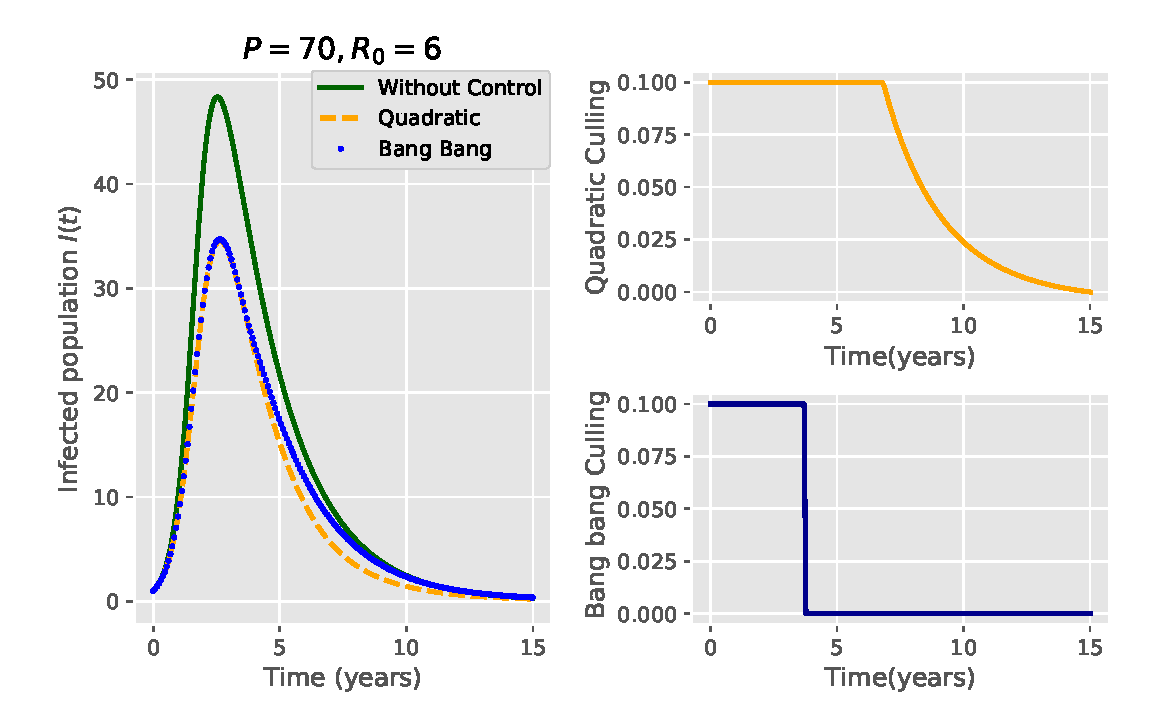
\includegraphics{Figures/figure_1_culling}
  \caption{State solutions without control, under optimal quadratic control 
  and with linear (bang-bang) control.}
  \label{fig:figure1culling}
\end{figure}

\begin{figure}[H]
  \centering
  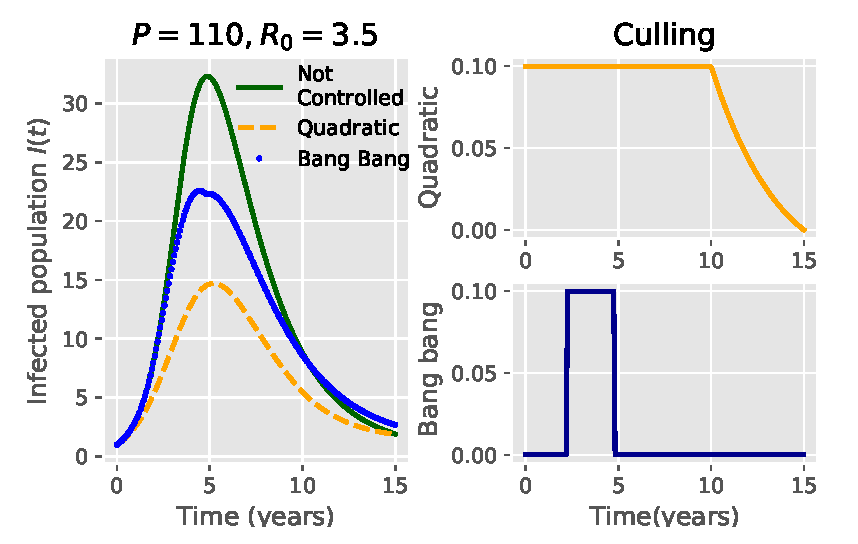
\includegraphics{Figures/figure_2_culling}
  \caption{State solutions without control, under optimal quadratic control 
  and with linear (bang-bang) control.}
  \label{fig:figure2culling}
\end{figure}

\begin{figure}[H]
  \centering
  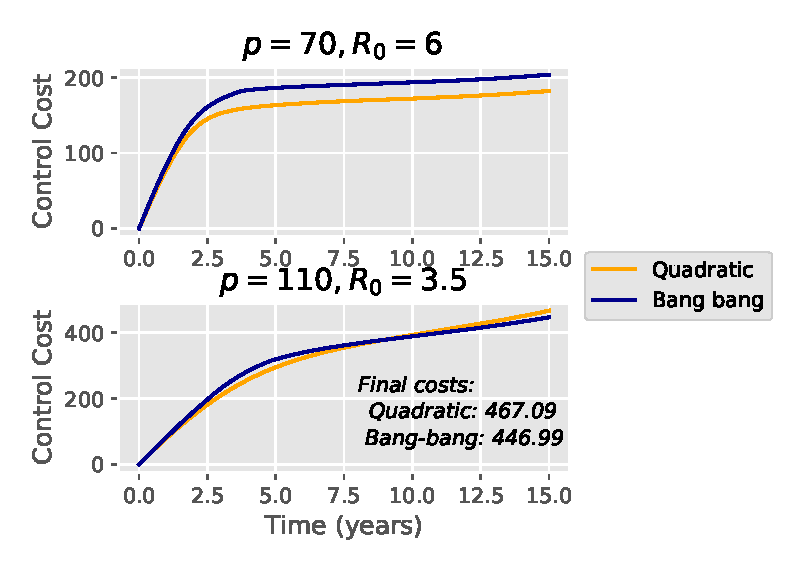
\includegraphics{Figures/figure_3_culling}
  \caption{Cost for the linear and quadratic controls under two scenes. Upper
  $P=70$, $R_0=6$, bottom, $P=110$, $R_0=3.5$, and the rest of parameters as 
  in \Cref{tbl:culling_par}.}
  \label{fig:figure3culling}
\end{figure}